% !TEX root = thesis.tex

%%
%%
%% Theoretical background chapter
%%
%%

%%%%%%%%%%%%%%%%%%%%%%%%%%%%%%%%%%%%%%%%%%%%%%%%%%%%%%%%%%%%%%%%%%%%%%%%%%%%%%
%%
%% Disease incidence
%%
%%%%%%%%%%%%%%%%%%%%%%%%%%%%%%%%%%%%%%%%%%%%%%%%%%%%%%%%%%%%%%%%%%%%%%%%%%%%%%
\section{Disease incidence}
\label{sec:theory:incidence}

The theory described in this section is based on \citet{rothman2008modern}.
We study chronic diseases in order to better understand the degree to which different groups of people are ``at risk'' of contracting a disease.
We also are interested in discovering and describing the association between environmental factors and this ``risk''.
For example, one could ask if air pollution emitted by a factory is associated with an increased ``risk'' of lung cancer among people that live close by.

In order to be more precise,
let us define

\begin{defn}
    \textbf{\Gls{risk}} is the probability of an individual person contracting a disease in a specific time period.
\end{defn}

One way to estimate the \gls{risk} is to look at the historical frequency of contracting of the disease.
The type of study we are interested in involves incidents of a chronic disease.
Therefore, we separately consider those people who contracted the disease under study.
In particular, we are interested in people who did not have the disease at the beginning of the study,
but developed the disease within the study period.
These are new cases of the disease, which we call \textbf{\glspl{incident}}.

\begin{defn}
    An \textbf{\gls{incident}} is a new case of the disease during the study period.
\end{defn}

The common measure of frequency used in the literature compares the number of new cases of a disease to the total time spent by members of the population in the study.
This measure is called the \gls{incidence rate}.

\begin{equation}
    \mbox{\Gls{incidence rate} (common definition)} = \frac{\mbox{number of new cases}}
                                {\displaystyle\smashoperator{\sum\limits_{\mbox{persons}}}\mbox{time spent by person in population}}
\end{equation}

For our simulation study, we can simplify our definition of \gls{incidence rate} by assuming that each person in the population is exposed for the entire study period,
which for simplicity we can set to one (1).
Our simplified definition of incidence rate is then:

\begin{defn}
    The \textbf{\gls{incidence rate}} is the number of new cases in the study period divided by the total population.
    \begin{equation}
        \label{eq:incidencerate}
        \mbox{\Gls{incidence rate}} = \frac{\mbox{number of new cases in a time period}}
                                        {\mbox{number of persons}}
    \end{equation}
\end{defn}

\Glspl{incidence rate} are always expressed in cases per person-time units.
For example, 10 cases of asthma per 100,000 people per year is a valid \gls{incidence rate}.

For a given population, time period, and set of \glspl{incident},
we can compute the overall \gls{incidence rate} by taking the total number of \glspl{incident} and dividing by the total population.
However, we may wish to compare the \gls{incidence rate} at different locations within an area.
To do this, we need to look at the number of cases and the population in the areas that are close to these locations.
If we then make these areas infinitesimally small,
then we could compute the \gls{incidence rate} point-wise.

\begin{defn}
    \label{defn:incidence_rate}
    The \textbf{point-wise \gls{incidence rate}} is a function that computes the local \gls{incidence rate} at a point by dividing the point-wise value of the number of new cases by the point-wise value of the population.
\end{defn}

From this point onwards, the term \gls{incidence rate} refers to the point-wise \gls{incidence rate}.

%%%%%%%%%%%%%%%%%%%%%%%%%%%%%%%%%%%%%%%%%%%%%%%%%%%%%%%%%%%%%%%%%%%%%%%%%%%%%%
%%
%% Spatial point processes
%%
%%%%%%%%%%%%%%%%%%%%%%%%%%%%%%%%%%%%%%%%%%%%%%%%%%%%%%%%%%%%%%%%%%%%%%%%%%%%%%
\section{Spatial point processes}
\label{sec:theory:spatial_point_processes}

The theoretical results in this section are taken from \citet{diggle1983spatial},
\citet{diggle1988equivalence},
\citet{guan2008consistent},
\citet{silverman1986density},
and \citet{wand1994kernel}.

In order to understand the geospatial patterns of disease incidence,
we consider points in two-dimensional space $\RS$.
We begin with

\begin{defn}
    A \textbf{study area} $\gls{W} \subset \RS$ is a region in the plane where we make observations.
\end{defn}

The observations we are interested in are points distributed in \gls{W} which we call \textbf{events}.

\begin{defn}
    \label{defn:event}
    An \textbf{event} is a point $\xvec \in \RS$, situated in a study area \gls{W} that we are interested in observing.
\end{defn}

For example, in the study area of the boundaries of a city, we consider the events of the addresses of the residents.
We call this set of events

\begin{defn}
    The \textbf{population} \gls{P} is the set of home address events of the residents of the study area \gls{W}.
\end{defn}

In general, we are interested in understanding the mechanism by which the events occurred.
We are interested both in the number of events, and even more so in the pattern by which their locations are distributed in \gls{W}.
Taking a spatial statistical approach, we model the underlying mechanism that generates events using the following:

\begin{defn}
    A \textbf{\gls{spp}} $\boldsymbol{\gls{Lambda}}$ is a stochastic mechanism which generates a random set of events.
\end{defn}

Suppose we have a \gls{spp} \gls{Lambda} on a study area $\gls{W} \subset \RS$.
We can count the total number of \glspl{event} and divide it by the total area of \gls{W}.
This gives us a quantity we call the \textbf{average \gls{intensity}} of \gls{Lambda}.
Sometimes the points are spread uniformly throughout \gls{W}.
In that case, we say that \gls{Lambda} is a homogeneous point process.
On the other hand, it is often the case that \gls{Lambda} is not uniform,
and we call it a heterogeneous point process.
When \gls{Lambda} is heterogeneous,
we would like to know the average \gls{intensity} around different points in \gls{W}.
For this
we define $\ds$ as an infinitesimal area around the point $\xvec$,
and $N\!(\ds)$ as the number of \glspl{event} inside $\ds$.
Then the \textbf{\gls{intensity}} $\boldsymbol{\gls{lambda}\xvec}$ at $\xvec \in \RS$ is

\begin{equation}
    \label{eq:lambda_differential}
    \lambda \xvec := \lim_{|\ds| \to 0}
        \left\{
            \frac{\mathbb{E}[N\!(\ds)]}% /
            {|\ds|}
        \right\}
\end{equation}

We can think of $\gls{lambda}\xvec \!\! \ds$ as the approximate probability of the infinitesimal area \ds~ containing a single \gls{event}.
Qualitatively, an intensity function differs from a probability density function in that it does not necessarily integrate to $1$.
In particular, we can write $\gls{lambda}$ as a scaled probability density function
where $f$ is a probability density function and \gls{mu} is a constant.

\begin{equation}
    \label{eq:lambda_mu}
    \gls{lambda}\xvec = \mu f\!\xvec
\end{equation}

For a point-wise \gls{incidence rate} function,
we compute two separate \gls{intensity} functions.
The first \gls{intensity} returns the point-wise expected number of cases of the disease,
while the second returns the point-wise population density.
Dividing the value obtained from first by the value obtained from the second results in the \gls{incidence rate} described in \Cref{defn:incidence_rate}.

%%%%%%%%%%%%%%%%%%%%%%%%%%%%%%%%%%%%%%%%%%%%%%%%%%%%%%%%%%%%%%%%%%%%%%%%%%%%%%
%%
%% Kernel estimation of the intensity
%%
%%%%%%%%%%%%%%%%%%%%%%%%%%%%%%%%%%%%%%%%%%%%%%%%%%%%%%%%%%%%%%%%%%%%%%%%%%%%%%%
\section{Kernel estimation of the intensity}
\label{sec:theory:kernelestimation}

This section is based on \citet{silverman1986density} and \citet{wand1994kernel}.
The usual case in practice is to start with a set of \glspl{event} that have been observed in a study area.
For example, we can have new cases of a disease in a city that were diagnosed over the course of a defined time period.
By our \Cref{defn:event},
we consider the location coordinates such as those of the home addresses of the people who were diagnosed.
Our goal is to estimate the \gls{intensity} function for disease cases using these observed \glspl{event}.
Similarly for the population,
we would like to estimate the population \gls{intensity} function.

A common method for estimating \gls{intensity} functions is known as
\textbf{\gls{kernel intensity estimation}}.
This technique utilizes a special function known as a \textbf{\gls{kernel}},
denoted by $\gls{K}\xvec$,
that satisfies

\begin{align}
    \gls{K}\xvec \ge 0~ \forall \xvec \in W, \text{and} \label{eq:k_pos} \\%
    \iintW{\gls{K}\xvec} & = 1 \label{eq:k_1} \text{.}%
\end{align}

\Cref{eq:k_pos,eq:k_1} are equivalent to stating that \Kdots~is a probability density on $\RS$.
Starting with a set of \glspl{event} $\gls{N} \subset \RS$,
and a positive value \gls{h} known as the bandwidth,
we define the the \gls{kernel intensity estimator} as follows:

\begin{defn}
    \label{defn:lambda_hat}
    The \textbf{\gls{kernel intensity estimator}} $\gls{lambda_hat}_h \xvec$
    is a technique for estimating the \gls{intensity} of an \gls{spp}
    from observed \glspl{event} \gls{N}.
    The formula for computing the \gls{kernel intensity estimator} is:
    \begin{equation}
        \label{eq:lambda_hat}
        \gls{lambda_hat}_h \xvec%
            = \sumS{\gls{K}\left( \frac{\xvec-(s_1, s_2)}{h} \right)} \text{.}%
    \end{equation}
\end{defn}

Where $\xvec-(s_1, s_2)$ is ordinary vector subtraction,
and $\frac{\xvec-(s_1, s_2)}{h}$ is scalar multiplication by $\frac{1}{h}$.
For the remainder of this section we treat $h$ as a scalar for ease of explanation.
However, with no loss of generality we will use separate bandwidths in each coordinate,
that is $\mathbf{h}=(h_1, h_2)$.

This is a natural extension to $\RS$ of the one dimensional \gls{kernel intensity estimator} $\gls{lambda_hat}_{1,h}$,
which has the formula

\begin{equation}
    \label{eq:lambda_hat_1}
    \gls{lambda_hat}_{1,h} = \sumSone{K_1\left( \frac{x - s}{h} \right)} \text{.}%
\end{equation}

Here, $K_1(x)$ is a one-dimensional kernel function.

In order to compute \gls{lambda_hat} using \Cref{eq:lambda_hat},
there are two choices to be made: the choice of the bandwidth \gls{h}
and the choice of \gls{kernel} \gls{K}.
The role of the \gls{kernel} function \Kdots~is to smooth the information obtained
from the observed \glspl{event} to an area around their locations.
Choosing different \glspl{kernel} results in different shapes to this smoothing.
However, this has only a small effect on the resulting \gls{intensity} estimate.
On the other hand,
the choice of bandwidth \gls{h} has a major effect on the \gls{intensity} estimate.
The bandwidth controls the width of the area smoothed by the \gls{kernel} function and hence on the overall amount of smoothing.

\Cref{fig:theory:kernel1d} shows an example of how \gls{kernel} smoothing works in  one-dimension for three different bandwidths.
The two-dimensional case is analogous.
The dots along the bottom are the observed \glspl{event}.
The dashed lines show the \gls{kernel} functions around each of these \glspl{event},
while the upper solid line is the \gls{intensity} estimate produced using \Cref{eq:lambda_hat_1}.
\Cref{fig:theory:kernel1d:02} shows the estimate with $h=0.2$.
It has two local modes, each with a bit of fluctuation at the peaks.
In \Cref{fig:theory:kernel1d:04} we still see two modes with $h=0.4$, but with smoother peaks.
\Cref{fig:theory:kernel1d:08} has smoothed the two peaks together into a single,
large peak by using the larger bandwidth of $h=0.8$.

\begin{figure}[htbp]
    \centering
    \begin{subfigure}[t]{0.32\textwidth}
        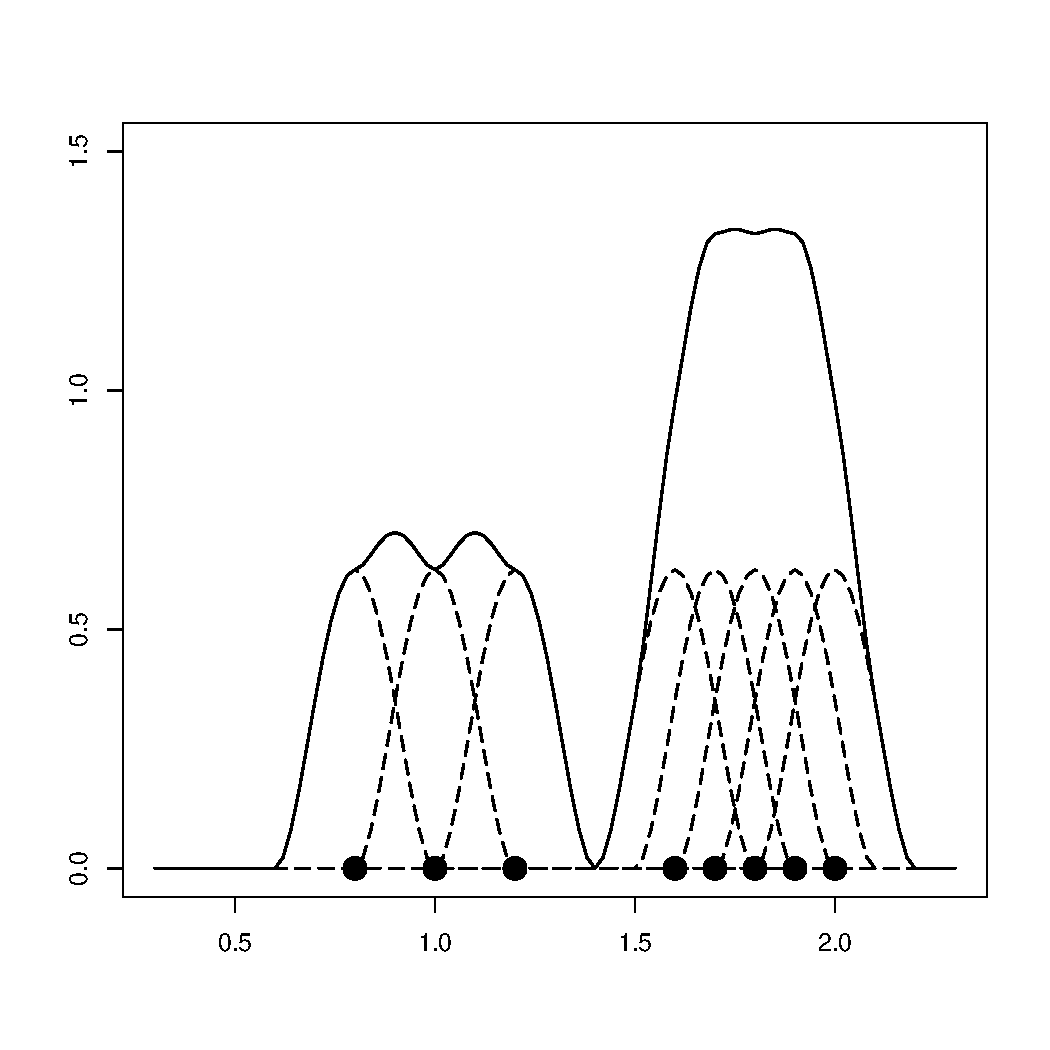
\includegraphics[width=\textwidth]{img/kernel1d-02}
        \subcaption{$h=0.2$}
        \label{fig:theory:kernel1d:02}
    \end{subfigure}
    \begin{subfigure}[t]{0.32\textwidth}
        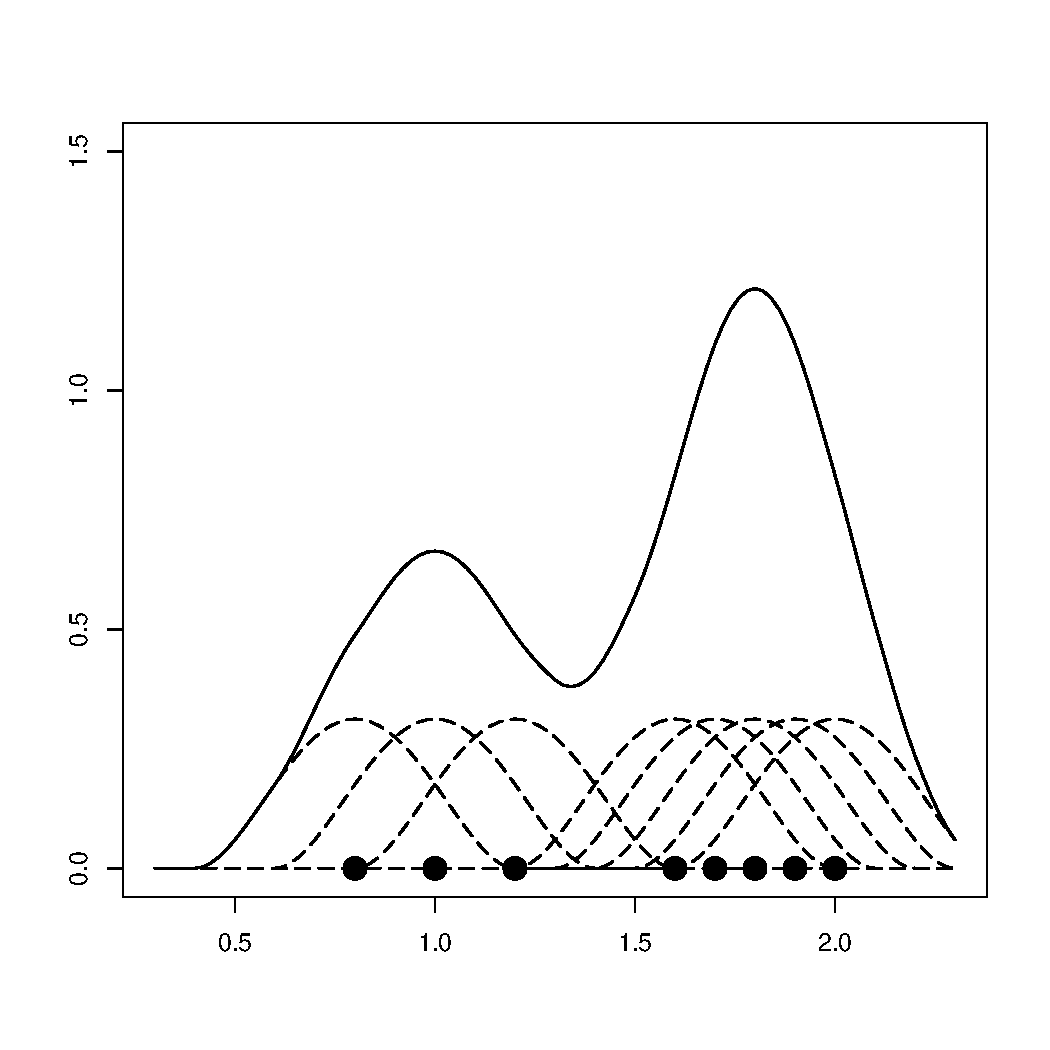
\includegraphics[width=\textwidth]{img/kernel1d-04}
        \subcaption{$h=0.4$}
        \label{fig:theory:kernel1d:04}
    \end{subfigure}
    \begin{subfigure}[t]{0.32\textwidth}
        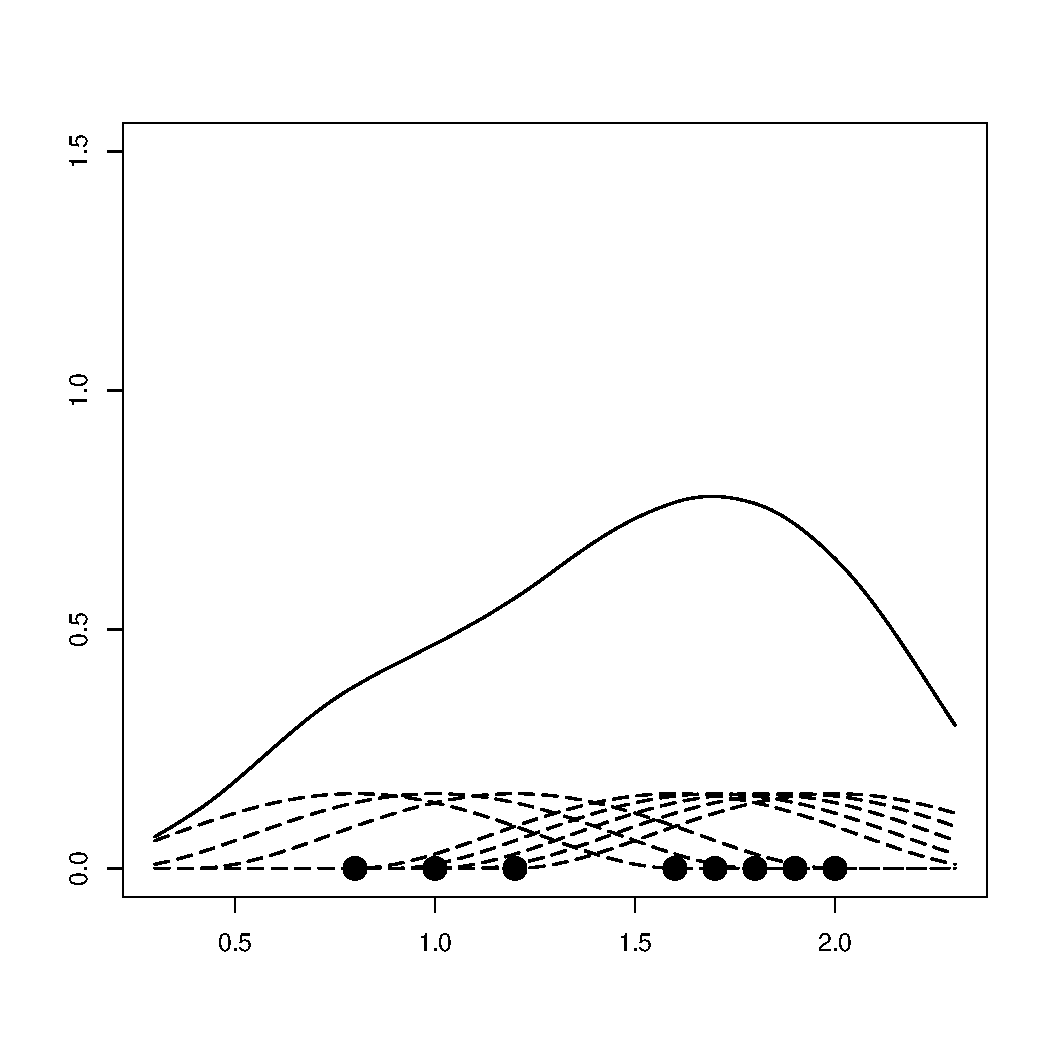
\includegraphics[width=\textwidth]{img/kernel1d-08}
        \subcaption{$h=0.8$}
        \label{fig:theory:kernel1d:08}
    \end{subfigure}
    \caption{One-dimensional \glsentryname{kernel} functions. The dots on the $x_1$ axis are the observed \glsentryplural{event}. The dashed lines are the kernel functions around these \glsentryplural{event} and the solid line is the \glsentryname{intensity} estimate $\hat{\lambda_1}$.}
    \label{fig:theory:kernel1d}
\end{figure}

In this study we use the two-dimensional biweight kernel found in \citet{silverman1986density} with formula
\begin{equation}
    \label{eq:biweightkernel2d}
    K \xvec =%
    \begin{cases}%
        \frac{3}{\pi}\left( 1 - x_1^2 - x_2^2 \right)^2 & \text{if}~x_1^2+x_2^2<1 \\%
        0 & \text{otherwise.}%
    \end{cases}%
\end{equation}

%%%%%%%%%%%%%%%%%%%%%%%%%%%%%%%%%%%%%%%%%%%%%%%%%%%%%%%%%%%%%%%%%%%%%%%%%%%%%%
%%
%% Measuring the accuracy of the estimate
%%
%%%%%%%%%%%%%%%%%%%%%%%%%%%%%%%%%%%%%%%%%%%%%%%%%%%%%%%%%%%%%%%%%%%%%%%%%%%%%%%
\section{Measuring the accuracy of the estimate}
\label{sec:theory:accuracy}

This section is based on \citet{silverman1986density} and \citet{wand1994kernel}.
A common statistical problem is to find the ``best'' estimate \gls{lambda_hat}
for the \gls{intensity} of an unknown \gls{spp}
based on a set of observed \glspl{event}.
In order to do this using \gls{kernel intensity estimation},
we must select the ``best'' bandwidth.
From \Cref{fig:theory:kernel1d} we can see that different values of bandwidth \gls{h} result in different estimates for the \gls{intensity}.
Our goal is to find a decision procedure that gives us the ``best'' result.
While there is a great deal of research in \gls{kde},
there is much less work available for \gls{kernel intensity estimation}.
We make use of one such result:
the optimal bandwidth used for computing the \gls{kernel intensity estimator} is the same as that for computing the related \gls{kde} function,
and can be determined by the same techniques \Citep{diggle1988equivalence}.
However, the \gls{kde} is used to estimate a probability density function,
while the \gls{kernel intensity estimator} is used to compute an intensity function.
Computationally, the difference is that a density must integrate to one,
and in order to do that,
we divide by $n$,
the number of observed events.


The first thing we must do is define what we mean by the ``best'' result.
We do this by choosing a measure of accuracy for the estimate,
and selecting the bandwidth which gives the optimal value for this measure.
One common accuracy measure used for function estimation is the \gls{mise},
because it has several useful mathematical properties.
It allows for additional analysis by being broken down into the mean integrated squared bias and mean integrated variance.
It can also be estimated by \acrlong{cv}.

Given a realized estimate \gls{lambda_hat} for any function \gls{lambda},
we can compute the squared error at any given point $\xvec \in \RS$ as
$\left( \lmbdhat - \lmbd \right)^2$,
and its expected value at $\xvec$ is called the \gls{mse}.
However,
we would like to compute the accuracy of the whole function.
We do this by integrating the squared error of the estimate over the study area to obtain the \gls{ise}.
\begin{equation}
\label{eq:ise}
    \mbox{\gls{ise}}(\gls{lambda_hat}) = \iintW{
            \left( \lmbdhat - \lmbd \right)^2
    }
\end{equation}
The \gls{mise} is the expected value of the \gls{ise} over the sample space of realizations of \gls{Lambda}.
\begin{align}
    \mbox{\gls{mise}}(\gls{lambda_hat}) 
        & = \E [\mbox{\gls{ise}}(\gls{lambda_hat})] \nonumber \\
        & = \E \iintW{ \left( \lmbdhat - \lmbd \right)^2 } \label{eq:mise}
\end{align}
The integrand of \Cref{eq:mise} is non-negative.
Therefore, by Fubini's Theorem, we can change the order of integration and expectation.
\begin{align}
    \mbox{\gls{mise}}(\gls{lambda_hat}) 
        & = \iintW{ \E \left( \lmbdhat - \lmbd \right)^2 } \nonumber \\
        & = \iintW{ \mbox{\gls{mse}}(\gls{lambda_hat}, \xvec) } \nonumber
\end{align}

We decompose \gls{mse} into the squared bias and squared variance (\Cref{eq:mse:biasvariance}),
giving us
\begin{align}
    \mbox{\gls{mise}}(\gls{lambda_hat}) 
        & = \iintW{ \Big( \E\lmbdhat - \lmbd \Big)^2 } \nonumber \\
        & \qquad + \iintW{ \E \Big( \lmbdhat - \E\lmbdhat \Big)^2 } \label{eq:mise:intbiasvariance}
\end{align}
We call the first part of \Cref{eq:mise:intbiasvariance} the \gls{isb} and the second part the \gls{iv}.

%%%%%%%%%%%%%%%%%%%%%%%%%%%%%%%%%%%%%%%%%%%%%%%%%%%%%%%%%%%%%%%%%%%%%%%%%%%%%%
%%
%% Asymptotic behavior of the bandwidth
%%
%%%%%%%%%%%%%%%%%%%%%%%%%%%%%%%%%%%%%%%%%%%%%%%%%%%%%%%%%%%%%%%%%%%%%%%%%%%%%%
\section{Asymptotic behavior of the bandwidth}
\label{sec:theory:asymptotic_bandwidth}

For the \gls{kernel intensity estimator},
the \gls{mise} cannot be computed directly.
Instead,
we approximate the bias,
the variance,
and finally the \gls{amise} which is the sum of the variance and the square of the bias.
In \Cref{sec:derivations:biasvariancekernel} we derive the \gls{amise}
for the \gls{kde}:
\begin{equation}
    \label{eq:amise}
    \mbox{\gls{amise}}(\hat{f}; h) = 
        \frac{1}{4} h^{4} \alpha^2 \iintW{\left( \nabla^2 f \xvec \right) } +
        n^{-1} h^{-2} \beta
\end{equation}
where
\begin{align}
    \alpha & = \iintR{x_1^2 K(x_1,x_2)} \\
    \beta & = \iintR{K(x_1,x_2)^2} \\
    \nabla^2 f \xvec & = \frac{\diffsq{f}\xvec}{\diff{x_1^2}} + \frac{\diffsq{f}\xvec}{\diff{x_2^2}} \text{.}
\end{align}

We can now take the derivative of \Cref{eq:amise} by $h$ and set it to zero,
giving us the optimal bandwidth \gls{h_opt}:
\begin{align}
    \gls{h_opt} & = C n^{-\frac{1}{6}}
\end{align}
where $C$ is a constant that depends on $f$ and $K$.
\begin{defn}
    The \gls{mise} \textbf{optimal bandwidth} $\mathbf{\gls{h_opt}}$ is the value of $h$ that minimizes the \gls{mise} of the \gls{kde} for a given distribution function $f$ and kernel function $K$.
\end{defn}
As noted above,
the optimal bandwidth of the \gls{kde} in the \gls{mise} sense is the same for the \gls{kernel intensity estimator}.

There are other accuracy measures that can be used to evaluate the estimate of the \gls{kernel intensity estimator}.
We discuss some of these in \Cref{sec:method:accuracy}.
Although we use these measures to characterize the behavior of the \gls{kernel intensity estimator} and the \gls{dkd},
our bandwidth is chosen by techniques that try to achieve \gls{h_opt} and minimize \gls{mise}.
However, as noted above,
our approximation \gls{amise} depends on the true function $f$.


%%%%%%%%%%%%%%%%%%%%%%%%%%%%%%%%%%%%%%%%%%%%%%%%%%%%%%%%%%%%%%%%%%%%%%%%%%%%%%
%%
%% Bandwidth selection from data
%%
%%%%%%%%%%%%%%%%%%%%%%%%%%%%%%%%%%%%%%%%%%%%%%%%%%%%%%%%%%%%%%%%%%%%%%%%%%%%%%
\section{Bandwidth selection from data}
\label{sec:theory:bandwidthselection}

In practice,
we don't know the true density or intensity functions.
Therefore we need cannot compute  \gls{h_opt},
\gls{mise} directly.
We use techniques that give us approximations for these values.
The two techniques we use are optimized to find a bandwidth that minimizes \gls{mise}.
The selected bandwidth may or may not be close to \gls{h_opt},
depending on the particular sample.

The first technique we will use is known as \textbf{\Gls{silverman}'s Rule of Thumb}.
We use the version for selecting bandwidth in $\RS$,
which has forumula
\begin{equation}
    \label{eq:silverman}
    h_S = 2.04 * \sigma * n^{-1/6}%
\end{equation}
where $n$ is the observed number of incidents,
$\sigma$ the arithmetic mean of the standard deviations of the $x_1$ and $x_2$ coordinates of the sample points.
\citet{silverman1986density} shows that for a large class of intensity functions,
including ones based on Gaussian functions,
this bandwidth provides a good approximation to the optimal bandwidth \gls{h_opt}. 

Our second technique is to use leave-one-out \textbf{\gls{cv}} over a set of bandwidths.
We select the bandwidth which minimizes the \gls{cv} error,
which approximates the \gls{mise}.
For the \gls{kde}, the formula for the \gls{cv} error of bandwidth $h$ for \gls{lambda_hat} is
\begin{equation}
    \mbox{\Gls{cv}}%
        = \iintW{\hat{f}_h \xvec^2}
        - 2 n^{-1} \sum\limits_{i=1}^n \hat{f}_{-i,h}\xvec%
\end{equation}
where $\hat{f}_{-i,h}\xvec$ is the \gls{kde} computed using the bandwidth $h$ and leaving out the $i^\text{th}$ point.
\Citet{brooks1991asymptotic} show that the \gls{cv} error computed with the selected bandwidth approximates the \gls{mise} very well,
and the ratio $\frac{\mbox{\gls{cv}}}{\mbox{\gls{mise}}} \to 1$ as $n$ increases.

The technique for \gls{kernel intensity estimation} is identical to the \gls{kde},
in the sense that the bandwidths which minimize the \gls{mise} of the \gls{kernel intensity estimator} are the same. 

%%%%%%%%%%%%%%%%%%%%%%%%%%%%%%%%%%%%%%%%%%%%%%%%%%%%%%%%%%%%%%%%%%%%%%%%%%%%%%
%%
%% Inconsistency of the kernel intensity estimator
%%
%%%%%%%%%%%%%%%%%%%%%%%%%%%%%%%%%%%%%%%%%%%%%%%%%%%%%%%%%%%%%%%%%%%%%%%%%%%%%%
\section{Inconsistency of the kernel intensity estimator}
\label{sec:theory:inconsistency}

This section is based on \citet{guan2008consistent}.
The \gls{kernel intensity estimator} above is not consistent,
in the sense that the \gls{mise} does not go to zero as the number of observed events $n$ increases.
We recall from \Cref{eq:amise},
that the \gls{amise} is composed of two terms.
The first term is proportional to $h^4$ while the second is proportional to $h^{-2}$.
Since the optimal bandwidth \gls{h_opt} is proportional to $n^{-\frac{1}{6}}$,
we see that the first term,
which is the asymptotic bias,
is $O(n^{-\frac{2}{3}})$.
However the second term,
which is the asymptotic variance is $O(n^{\frac{1}{3}})$ which does not go to zero as $n$ increases.

%%%%%%%%%%%%%%%%%%%%%%%%%%%%%%%%%%%%%%%%%%%%%%%%%%%%%%%%%%%%%%%%%%%%%%%%%%%%%%
%%
%% Estimation of the mode
%%
%%%%%%%%%%%%%%%%%%%%%%%%%%%%%%%%%%%%%%%%%%%%%%%%%%%%%%%%%%%%%%%%%%%%%%%%%%%%%%
\section{Estimation of the mode}
\label{sec:theory:mode}

This section is based on \citet{bickel2006fast} and \citet{hedges2003comparison}.
Often, one of the goals of intensity estimation is to find the point with the greatest \gls{risk} of coming down with a particular disease.
Mathematically, the point where this occurs in a probability distribution is called the mode.
For intensity, we refer to it as the peak and it is the point where the true intensity function takes its highest value.
However, when it comes to estimating the peak,
using the point with the highest value does not always give good results,
having both high bias and high variance.
There are some techniques, such as those described in \citep{dalenius1965mode},
which provide more stable estimates.
In addition to the computing the simple peak, use a simplified version of one of Dalenius' methods.
We take the highest five percent of the estimated intensity,
and find its center of mass.
This point $\xvec$~and the value of the estimate $\gls{lambda_hat} \xvec$ are our estimate of the peak.
We expect that this will give us a more stable estimate of where the disease risk is highest.

%%%%%%%%%%%%%%%%%%%%%%%%%%%%%%%%%%%%%%%%%%%%%%%%%%%%%%%%%%%%%%%%%%%%%%%%%%%%%%
%%
%% Data generation process
%%
%%%%%%%%%%%%%%%%%%%%%%%%%%%%%%%%%%%%%%%%%%%%%%%%%%%%%%%%%%%%%%%%%%%%%%%%%%%%%%
\section{Data generation process}
\label{sec:theory:data}

We generate data for each experiment as follows.
Before we begin, we set the random number seed to a fixed value for all experiments.
The first step is to generate a population.
We choose a distribution function $f_p$ over \gls{W},
and scale it to obtain an the population intensity function \gls{lambda_p} of a \gls{spp} \gls{Lambda} with an expected number of points the same as our chosen population size.
This means that the actual population size may not be exactly what we have chosen.
We then generate points $\xvec$ uniformly in \gls{W} and keep them with probability \gls{lambda_p}$\xvec$.
This gives us our population \gls{P} which use throughout the experiment.
In this way,
if \gls{lambda_p}$\xvec$ has twice the value of \gls{lambda_p}$(y_1, y_2)$ for two points $\xvec$ and $(y_1, y_2)$ in \gls{W},
then we expect to see about twice as many points around $\xvec$ than around $(y_1, y_2)$ in \gls{P}.

Once we have a fixed population, we have need to decide which members of the population constitute the incidents.
The process to generate the incidents is similar to that of the population.
We create an incident intensity function \gls{lambda_i} of a \gls{spp} for incidents.
We then take the points $\xvec \in \gls{P}$ and keep each one with probability \gls{lambda_i}$\xvec$.
This gives us our set of incidents \gls{I}.
Once again, when \gls{I}$\xvec$ is higher than \gls{I}$(y_1, y_2)$,
then the probability of $\xvec \in \gls{I}$ is correspondingly higher than that of $(y_1, y_2)$.

